\documentclass[11pt,a4paper,titlepage]{article}

% Font related packages
\usepackage{fontspec}
\setmainfont{Lato}
\setsansfont{Lato}
\setmonofont{Fira Mono}
\newfontfamily\greekfont[Script=Greek]{Lato}

% Greek monospace font
\newfontfamily{\greekfonttt}{Fira Mono}
\usepackage{polyglossia}
\setdefaultlanguage{greek}

% Math packages
\usepackage{amsmath}
\usepackage{amsfonts}
\usepackage{amssymb}
\usepackage{makeidx}
\usepackage{eurosym}

% Graphics
\usepackage{graphicx}
\usepackage{float}
\usepackage{tikz}
\usetikzlibrary{arrows,positioning,shapes}

\usepackage{appendix} % Add appendix to document
\usepackage[margin=3cm]{geometry} % Change page margins

% Table packages
\usepackage{multirow}
\usepackage{color, colortbl}
\usepackage{array}
\usepackage{longtable}
\usepackage{lscape}

% PDF options
\usepackage[unicode,hidelinks,pdftitle={Ανάπτυξη συστήματος με υλοποίηση μεθοδολογίας MINORA (UTA) σε περιβάλλον Python με web interface},pdfauthor={Dimitrios Maroulidis, Myron Pachakis},pdfcreator={},pdfproducer={}]{hyperref}

% Colors to use in tables
\definecolor{LightGray}{gray}{0.95}
\definecolor{Gray}{gray}{0.9}
\definecolor{LightRed}{HTML}{ff6b6b}
%\definecolor{LightBlue}{HTML}{aacfff}
%\definecolor{LightBlue}{HTML}{5eaeff}
\definecolor{LightBlue}{HTML}{a7d2ff}

% Table column types for math environments
\newcolumntype{e}{>{$}c<{$}}
\renewcommand{\arraystretch}{1.2}
\usepackage{ragged2e}

% Math font
\usepackage{unicode-math}
\setmathfont{Asana Math}
% Use section based numbering for equations.
% amsmath is needed for this.
\numberwithin{equation}{section}

% Use comma as decimal point
%\usepackage{icomma}

% Code highlighting
\usepackage{minted}

% Comments
\usepackage{comment}

\author{Δημήτριος Μαρουλίδης (\textit{2018010111}) \and
    Μύρων Παχάκης (\textit{2018010028})}
\title{Ανάπτυξη συστήματος με υλοποίηση μεθοδολογίας MINORA (UTA) σε περιβάλλον Python με web interface}
\date{\today}

\begin{document}
\maketitle	
\tableofcontents
%	\listoffigures
%	\listoftables

\clearpage
% BEGIN HERE

\begin{comment}
Πλάνο Σύνταξης Αναφοράς
Εισαγωγή
1.Αντικειμενικοί Στόχοι Εργασίας-Προγράμματος
2.Περιγραφή μεθόδου θεωρητικά (Λογική της μεθόδου, ποιός την έφτιαξε)
3.Αναλύτικη Περιγραφή Μεθόδου (Χρησιμοποιούμε αυτό, κάνουμε αυτό, παρουσίαση αποτελέσματος, δεν σταματάμε όμως εκεί έχουμε ανατροφοδότηση από τον χρήστη (web interface), κάνει αυτή τη διαδικασία ο χρήστης)
4.Περιγραφή Υλοποίησης
5.Αναλυτικό Παράδειγμα εφαρμογής της μεθόδου
6.Παράρτημα -> Οδηγίες Χρήσης του προγράμματος-μεθόδου
7.Συμπεράσματα
8.Βιβλιογραφία
\end{comment}

\begin{abstract}
Η εργασία παρουσιάζει τη δημιουργία ενός αλληλεπιδραστικού προγράμματος στη γλώσσα προγραμματισμού Python για την επίλυση πολυκριτήριων συστήματων υποστήριξης αποφάσεων χρησιμοποιώντας το σύστημα MINORA. Για την υλοποίηση του συστήματος MINORA θα γίνει, επίσης, χρήση της μεθόδου πολυκριτήριας ανάλυσης UTASTAR. 

Η εργασία χωρίζεται σε δύο μέρη, το θεωρητικό αποτελείται από τα Κεφάλαια (1-3) και το προγραμματιστικό από τα Κεφάλαια (4-7). Στο Κεφάλαιο \ref{sec:goals} παρουσιάζονται οι αντικειμενικοί στόχοι που αναμένονται από το πρόγραμμα. Στο Κεφάλαιο \ref{sec:theory} περιγράφεται αναλυτικά η θεωρία πίσω από την μέθοδο UTASTAR και το σύστημα MINORA όπως η λογική λειτουργίας και ο τρόπος χρήσης τους, καθώς και οι πρωτοπόροι υλοποίησης και παρουσίασης των μεθόδων. Στο Κεφάλαιο \ref{sec:theory_in_depth} γίνεται αναλυτική παρουσίαση βήμα-βήμα στη εφαρμογή των μεθόδων UTA-UTASTAR-MINORA.

Στο Κεφάλαιο \ref{sec:implementation} αναλύεται διεξοδικά το πρόγραμμα σε γλώσσα Python καθώς και η αλληλεπίδραση μέσω του web interface, ενώ στο Κεφάλαιο \ref{sec:example} δίνεται ένα παράδειγμα πολυκριτήριων αποφάσεων και εφαρμόζεται η μέθοδος MINORA. Στο Κεφάλαιο \ref{sec:instructions} εντοπίζονται εκτενείς οδηγίες χρήσης του προγράμματος και στο Κεφάλαιο \ref{sec:} συνοψίζονται τα συμπεράσματα της εργασίας και της χρήσης των μεθόδων-προγράμματος. Στο Κεφάλαιο \ref{sec:} δίνεται η σχετική βιβλιογραφία και οι πηγές που χρησιμοποιήθηκαν.
\end{abstract}


%Μία πρώτη προσπάθεια είναι, δες ότι δεν σου αρέσει ή οτι θες να αλλάξουμε (πιθανών και να γραψουμε λιγα παραπανω?) Επίσης όπου υπάρχουν οι αριθμοί των κεφαλαίων θα αλλάξουν με τα tags των sectors για να μην γινεται μπερδεμα.  

\section{Αντικειμενικοί Στόχοι}
\label{sec:goals}   
\begin{itemize}
	\item Συγγραφή ενός προγράμματος σε γλώσσα προγραμματισμού Python με σκοπό την υποστήριξη για τη λήψη αποφάσεων από τον χρήστη.
	\item Υλοποίηση συστήματος MINORA της οποίας το αποτέλεσμα είναι ένα μοντέλο το οποίο μοντελοποιεί τη διαδικασία απόφασης όσο πιο πιστά γίνεται.
	\item Παρουσίαση σε απλή και ευανάγνωστη μορφή του αποτελέσματος.
	\item Δυνατότητα άμεσης αλληλεπίδρασης του χρήστη με το πρόγραμμα μέσω web interface.
	\item Επίδειξη αναλυτικών οδηγιών χρήσης του προγράμματος.
\end{itemize}


\section{Θεωρητική Περιγραφή Μεθόδου}
\label{sec:theory}
Η μέθοδος πολυκριτήριας ανάλυσης UTASTAR (UTilités Additives *) είναι υπεύθυνη για την εκτίμηση μίας ή παραπάνω συναρτήσεων αξίας χρησιμοποιώντας διαδικασίες γραμμικού προγραμματισμού. Στόχος των συναρτήσεων αξίας που θα εξαχθούν είναι η όσο το δυνατόν καλύτερη κατάταξη κάποιων επιλογών $a$ σε σύγκριση με την αρχική κατάταξη που έχει δωθεί από τον χρήστη. Ο χρήστης είναι υπεύθυνος για την εισαγωγή ενός συνόλου επιλογών $A_{R}$ κατανεμημένου με σειρά προτίμησης καθώς επίσης και ενός συνόλου κριτηρίων επιλογής $g_{n}$. 

Το σύστημα MINORA (Multicriteria Interactive Ordinal Regression Analysis), χρησιμοποιεί την μέθοδο UTASTAR για την εξαγωγή της λύσης του πολυκριτήριου προβλήματος, με την διαφορά ότι το σύστημα δίνει την δυνατότητα στον χρήστη να ανατροφοδοτήσει τυχόν δεδομένα, καταλήγοντας στο επιθυμητό σύστημα προτιμήσεων.

Πρωτοπόροι επιμελητές της μεθόδου UTASTAR είναι οι καθηγητές Siskos, Y. και Yannacopoulos, D., το 1985, ενώ το σύστημα MINORA επιμελήθηκε από τον καθηγητή Siskos, Y. και συνεργάτες, το 1993 και το 1994. 

%Δεν έχω αναφέρει πουθενά την UTA, θεωρείς ότι πρέπει να την αναφέρουμε?
\newpage

\section{Αναλυτική Περιγραφή Μεθόδου}
\label{sec:theory_in_depth}
\subsection{UTASTAR}
Όπως έχει ήδη ειπωθεί ο χρήστης παρέχει ένα σύνολο $A_{R}$ εναλλακτικών επιλογών $a$ κατανεμημένων με σειρά προτίμησης από το καλύτερο στο χειρότερο καθώς επίσης και ένα σύνολο κριτηρίων $g_{n}$. Ανάλογα με τον αριθμό των επιλογών, θα χωριστούν ισαπέχοντα διαστήματα για κάθε κριτήριο χωριστά: 

\begin{equation}\label{initial_inter}
[g_{i*},g^{*}_{i}] = [g^{1}_{i}, ..., g^{a_{i}}_{i}]
\end{equation}
όπου $g^{a_{i}}_{i}$ οι διάφορες τιμές του συγκεκριμένου κριτηρίου, $g_{i*}$ η χειρότερη τιμή του συγκεκριμένου κριτηρίου και $g^{*}_{i}$ η καλύτερη τιμή του συγκεκριμένου κριτηρίου. 	
Σε αυτό το σημείο είναι απαραίτητο να γίνει ορισμός της έννοιας των χρησιμοτήτων των διαφόρων επιλογών $u(g(a))$, ο οποίος αποτελεί το μοντέλο απόφασης στην μέθοδο UTASTAR. Eκφράζεται ως μία προσθετική συνάρτηση των αύξουσων μερικών χρησιμοτήτων των κριτηρίων $u_{i}(g^{j}_{i})$:

\begin{equation}\label{total_uti}
	u(g(a)) = \sum_{i=1}^{n} u_{i}(g_{i}(a)) = u_{1}(g_{1}(a)) + u_{2}(g_{2}(a)) + ... + u_{n}(g_{n}(a))
\end{equation}
όπου $i = 1,2,...,n$ ο αριθμός του κριτηρίου και $a\in A_{R}$ η συγκεκριμένη επιλογή.

Λόγω του ότι ο χρήστης έχει κατατάξει τις επιλογές του κατά σειρά προτίμησης τότε είναι προφανές ότι η επιλογή $a_{m}$ θα είναι πάντα προτιμότερη ή ίση (αδιάφορη) από την επιλογή $a_{m+1}$.    

Είναι, λοιπόν, απαραίτητο να διατηρηθεί η μονοτονικότητα των κριτηρίων $g_{i}$. Έτσι με βάση την προτιμησιακή ανεξαρτησία των κριτηρίων η μονοτονία παραμένει ίδια τόσο στις μερικές συναρτήσεις χρησιμοτήτων $u_{i}(g^{j}_{i})$ όσο και στην ολική συνάρτηση  $u(g(a))$.

\centerline{Σε περίπτωση προτίμησης ισχύει: $u_{i}(g^{j+1}_{i}) > u_{i}(g^{j}_{i})$}

\centerline{Σε περίπτωση αδιαφορίας ισχύει: $u_{i}(g^{j+1}_{i}) = u_{i}(g^{j}_{i})$}

Στη συνεχεία ορίζονται οι μεταβλητές $w_{ij}$ σύμφωνα με τις παραπάνω σχέσεις μονοτονίας των κριτηρίων ως:

\begin{equation}\label{def_w}
	w_{ij} = u_{i}(g^{j+1}_{i}) - u_{i}(g^{j}_{i}) \geq 0
\end{equation}
όπου $i = 1,2,...,n$ και $j = 1,2,...,a_{i}-1$. Με αυτόν τον τρόπο είναι δυνατόν να αναπαρασταθεί η εξίσωση \ref{total_uti} των ολικών χρησιμοτήτων $u(g(a))$ με χρήση των μεταβλητών $w_{ij}$ αντί με χρήση των μερικών χρησιμοτήτων $u_{i}(g^{j}_{i})$. 

Για να πραγματοποιηθεί αυτή η μετατροπή είναι απαραίτητο να γίνει χρήση των παρακάτω σχέσεων:

\begin{equation}\label{zero_crit}
	u_{i}(g^{1}_{i}) = 0
\end{equation}

\begin{equation}\label{sum_w}
	u_{i}(g^{j}_{i}) = \sum_{i=1}^{j-1} w_{ij}
\end{equation}
όπου $i = 1,2,...,n$ και $j = 2,3,...,a_{i}-1$.

\newpage

Η εξίσωση \ref{zero_crit} είναι υπεύθυνη για τον μηδενισμό της χειρότερης τιμής του κάθε κριτηρίου ενώ στην εξίσωση \ref{sum_w} παρουσιάζεται η τιμή της χρησιμότητας του κάθε κριτηρίου ως το άθροισμα των μεταβλητών $w_{ij}$.  

Εάν οποιαδήποτε μερική χρησιμότητα $u_{i}(g_{i}(a))$ δεν υπάρχει στις διακριτές τιμές του αντίστοιχου κριτηρίου τότε είναι αναγκαίο να γίνει γραμμική παρεμβολή στο συγκεκριμένο κριτήριο $g_{i}^{j}$. 

Θεωρούνται πεπερασμένα τα άκρα $g_{i*}$ και $g^{*}_{i}$ του κριτηρίου και γίνεται χωρισμός του διαστήματος από την σχέση \ref{initial_inter} σε ισάριθμα υποδιαστήματα $(a_{i}-1)$, όπου το συγκεκριμένο σημείο που θα γίνει ο χωρισμός υπολογίζεται από τον τύπο:

\begin{equation}
	g_{i}^{j} = g_{i*} + \frac{j-1}{a_{i}-1}(g^{*}_{i}-g_{i*})
\end{equation}
για $j = 1,2,...,a_{i}$ και $g_{i*}$ η χειρότερη τιμή του συγκεκριμένου κριτηρίου και $g^{*}_{i}$ η καλύτερη τιμή του συγκεκριμένου κριτηρίου.

Η γραμμική παρεμβολή εφαρμόζεται σύμφωνα με τον τύπο \ref{linear_inter} και δίνει ως αποτέλεσμα την τιμή της μερικής χρησιμότητας για την επιλογή $a$.

\begin{equation}\label{linear_inter}
	u_{i}(g_{i}(a)) = u_{i}(g^{j}_{i}) + \frac{g_{i}(a)-g^{j}_{i}}{g^{j+1}-g^{j}_{i}}(u_{i}(g_{i}^{j+1})-u_{i}(g_{i}^{j}))
\end{equation}


Στη μέθοδο UTASTAR είναι απαραίτητο να χρησιμοποιηθεί μία διπλή συνάρτηση σφάλματος όπου θα εκφράζει το ποσό της χρησιμότητας που θα πρέπει να προστεθεί ή να αφαιρεθεί, αντίστοιχα, από την ολική χρησιμότητα $u(g(a))$ με σκοπό να είναι δυνατόν η επιλογή $a$ που έχει ως ολική χρησιμότητα την $u(g(a))$ να ανακατακτήσει την θέση της στη διάταξη των επιλογών.

Τα 2 σφάλματα αυτά ονομάζονται σφάλμα υποεκτίμησης $σ^{+}$ το οποίο αφαιρεί ένα ποσό αξίας και σφάλμα υπερεκτίμησης $σ^{-}$ το οποίο προσθέτει ένα ποσό αξίας.

Με αυτόν τον τρόπο τα σημεία των επιλογών $a$ σταθεροποιούνται με μεγαλύτερη ακρίβεια πάνω στην καμπύλη μονότονης παλινδρόμησης όπως παρουσιάζεται στο σχήμα \ref{fig:graph_monot}.

\begin{figure}[H]
	\centering
	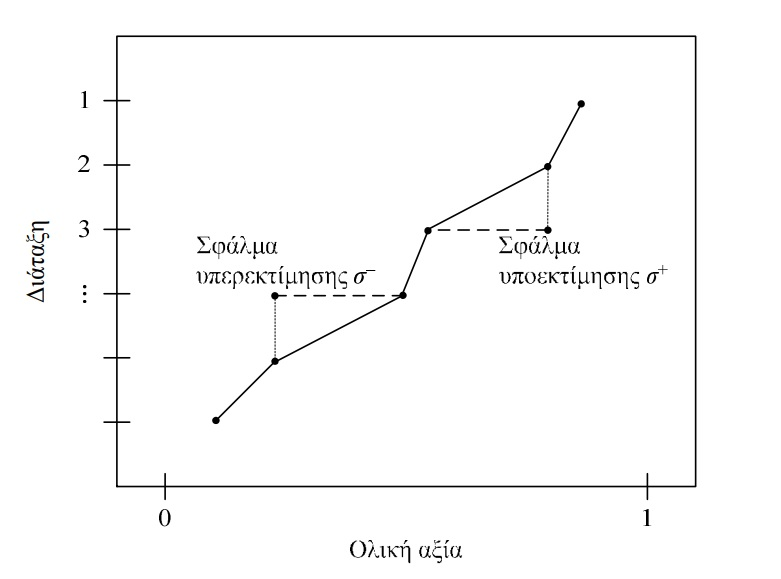
\includegraphics[width=0.7\linewidth]{media/graph_mono.jpg}
	\caption{Καμπύλη Μονότονης Παλινδρόμησης}
	\label{fig:graph_monot}
\end{figure}

Με τις παραπάνω προσθήκες των σφαλμάτων η εξίσωση των ολικών χρησιμοτήτων \ref{total_uti} μετατρέπεται σε:

\begin{equation}\label{total_uti_fin}
	u(g(a)) = \sum_{i=1}^{n} u_{i}(g_{i}(a)) - σ^{+}(a) + σ^{-}(a)
\end{equation}
όπου $i = 1,2,...,n$ ο αριθμός του κριτηρίου και $a\in A_{R}$ η συγκεκριμένη επιλογή.

Έτσι για δύο διαδοχικές επιλογές $a_{m}$ και $a_{m+1}$ ορίζεται:

\begin{equation}\label{def_deltas}
	Δ(a_{m}, a_{m+1}) = u(g(a_{m})) - σ^{+}(a_{m}) + σ^{-}(a_{m}) - u(g(a_{m+1})) + σ^{+}(a_{m+1}) - σ^{-}(a_{m+1})
\end{equation}

Όπου οι χρησιμότητες $u(g(a_{m}))$ μπορούν να αντικατασταθούν από τις μεταβλητές $w_{ij}$ με βάση τις σχέσεις \ref{def_w} και \ref{sum_w}.
 
Έχει ήδη αναφερθεί πως η μέθοδος UTASTAR χρησιμοποιεί μεθόδους γραμμικού προγραμματισμού για τον υπολογισμό των μερικών συναρτήσεων χρησιμότητας-αξίας. Επιλύεται το παρακάτω γραμμικό πρόβλημα (ΓΠ) με αντικειμενική συνάρτηση ελαχιστοποίησης των συνολικών σφαλμάτων $σ^{+}$ και $σ^{-}$.

\begin{equation}\label{linear_program}
	\begin{aligned}
	&min~F = \sum_{a\in A_{R}} {σ^{+}(a) + σ^{-}(a)} \\
	&\text{υπό περιορισμούς}\\
	&Δ(a_{m},a_{m+1}) \geq δ ~\text{εάν}~ a_{m}\succ a_{m+1}\\
	&Δ(a_{m},a_{m+1}) = 0 ~\text{εάν}~ a_{m}\sim a_{m+1}\\
	&\sum_{n}^{i=1}\sum_{j=1}^{a_{i}-1} w_{ij} = 1\\
	& w_{ij} \geq 0, σ^{+}(a) \geq 0, σ^{-}(a) \geq 0 \forall a\in A_{R}, \forall i,j
	\end{aligned}
\end{equation}
 
\newpage

Όπου $δ$ ορίζεται ως η τιμή του κατωφλιού προτίμησης και έχει μία μικρή θετική τιμή. Εξασφαλίζει ότι η διάταξη των εναλλακτικών ταιριάζει με το μοντέλο προτιμήσεων του αποφασίζοντα.

Αφού εξαχθεί η λύση του γραμμικού προγράμματος τότε γίνεται ανάλυση ευστάθειας, δηλαδή ελέγχουμε εάν υπάρχουν περισσότερες από μία βέλτιστες λύσεις ή εάν υπάρχουν λύσεις που είναι πολύ κοντά στη βέλτιστη που έχουμε υπολογίσει.

Σε περίπτωση όπου η βέλτιστη λύση της αντικειμενικής συνάρτησης έχει τιμή μηδέν τότε υπάρχουν παραπάνω από μία λύσεις που ικανοποιούν την διάταξη επιλογών $A_{R}$ που έχει εισάγει ο χρήστης. Τότε υπολογίζουμε τη μέση τιμή των συναρτήσεων χρησιμότητας εκείνων των κοντινότερων βέλτιστων λύσεων που μεγιστοποιούν τις αντικειμενικές συναρτήσεις:

\begin{equation}\label{eq:sens-analysis-Obj-Fun}
	u_{i}(g_{i}^{*}) = \sum_{j=1}^{a_{i}-1} w_{ij}  ~~\forall i=1,2,..,n
\end{equation} 

Η αντικειμενική συνάρτηση του αρχικού γραμμικού προγράμματος \eqref{linear_program} θέτεται ως περιορισμός:

\begin{equation}\label{eq:sens-analysis-constr}
	\sum_{a\in A_{R}} {σ^{+}(a) + σ^{-}(a)} \leq z^{*} + ε
\end{equation}

Όπου $z_{*}$ είναι η βέλτιστη τιμή του αρχικού γραμμικού \ref{linear_program}, δηλαδή το ελάχιστο σφάλμα, και $ε$ είναι είτε μηδέν είτε ένας μικρός θετικός αριθμός. 

Όταν υπάρχει αστάθεια οι βέλτιστες λύσεις των γραμμικών προγραμμάτων παρουσιάζουν μεγάλη απόκλιση μεταξύ τους, γεγονός το οποίο οδηγεί σε μεγαλύτερη διακύμανση των μεταβλητών $w_{ij}$. Με αυτόν τον τρόπο μπορούμε να καταλάβουμε πόσο σημαντικό είναι το κάθε κριτήριο $g_{i}$ στη διάταξη επιλογών που έχει ορίσει ο χρήστης.

Σε αυτό το σημείο έχει εφαρμοστεί η μέθοδος UTASTAR και έχουν εξαχθεί τα τελικά αποτελέσματα καθώς και η τελική κατάταξη των εναλλακτικών που προτείνει το σύστημα σύμφωνα με τη συνάρτηση χρησιμότητας.
Επιπλεόν σημαντικό είναι να οριστεί μία μεταβλητή η οποία θα προσδιορίζει την διαφορά της αρχικής προδιάταξης του χρήστη από την τελική προδιάταξη που προκύπτει από τη συνάρτηση χρησιμότητας. Αυτή η μεταβλητή ονομάζεται $τ$ του Kendall και κυμαίνεται στο διάστημα $[-1,1]$ όπου με τιμή $-1$ δεν υπάρχει καμία ομοιότητα ανάμεσα στις δύο κατατάξεις και με τιμή $1$ οι κατατάξεις ταυτίζονται.

\subsection{MINORA}
\label{ssec:minora-theory}
Όπως έχει ήδη αναφερθεί το σύστημα MINORA χρησιμοποιεί αυτά τα δεδομένα-αποτελέσματα και επιτρέπει στον χρήστη να προβεί σε διάφορες ενέργειες-αναδράσεις έτσι ώστε να υπάρχει απόλυτη συμφωνία ανάμεσα στη αρχική προδιάταξη και στη διάταξη του μοντέλου.

Παρακάτω συνοψίζονται οι διαφορετικές αναδράσεις με τις οποίες ο χρήστης μπορεί να επιτύχει απόλυτη συμφωνία. Η προτίμηση κάποιας εκ των αναδράσεων είναι αποκλειστικά επιλογή του χρήστη-αποφασίζοντα.

\begin{description}
	\item[Ανάδραση τύπου 1]
	Ο χρήστης αρνείται να μεταβάλει την σειρά προτίμησης των εναλλακτικών ώστε να ταυτίζεται με το τελικό μοντέλο και συνεπώς διαφοροποιεί τη μοντελοποίηση των κριτηρίων:
	\begin{itemize}
		\item Είτε ενώνοντας δύο παρόμοια κριτήρια σε ένα κοινό
		\item Είτε χωρίζοντας ένα σύνθετο κριτήριο σε δύο 
		\item Είτε αλλάζοντας το διάστημα που κυμαίνεται ένα ή περισσότερα κριτήρια
		\item Είτε προσθέτοντας καινούργιο κριτήριο ή κριτήρια
		\item Είτε διαγράφοντας ένα ή και περισσότερα κριτήρια
	\end{itemize}
	Σε κάθε μία από τις παραπάνω περιπτώσεις ο αποφασίζων επαναχρησιμοποιεί τη μέθοδο UTASTAR για να γίνει επίλυση του καινούργιου προβλήματος με τις διαφορετικές μεταβλητές.
	\item[Ανάδραση τύπου 2]
	Σε αυτή την περίπτωση ο χρήστης θεωρεί σωστό το τελικό μοντέλο και αλλάζει την κρίση του έτσι ώστε να ταυτίζεται με τα αποτελέσματα του μοντέλου.	
	\item[Ανάδραση τύπου 3]
	Παρομοίως με την ανάδραση 1 ο χρήστης διαφωνεί με το τελικό μοντέλο κατάταξης αντί όμως να γίνει αλλαγή στα κριτήρια, μεταβάλλονται οι μερικές χρησιμότητες των κριτηρίων στα σημεία όπου είναι δυνατόν να πραγματοποιηθεί αυτό. Όπως είναι λογικό θα προκύψει διαφορετική συνάρτηση χρησιμότητας και ο χρήστης εφαρμόζει ξανά την μέθοδο UTASTAR για να ελεγχθεί τυχών νέα ασυμφωνία.   
	\item[Ανάδραση τύπου 4]
	Όταν δεν υπάρχει καμία απολύτως συμφωνία ανάμεσα στο τελικό μοντέλο και στη προδιάταξη τότε είναι απαραίτητο να γίνει απόρριψη του τρέχοντος μοντέλου ανάλυσης και να δημιουργηθεί ένα καινούργιο από την αρχή.
	\item[Ανάδραση τύπου 5]
	Πλήρης συμφωνία ανάμεσα στο μοντέλο και την προδιάταξη του χρήστη οδηγεί σε εφαρμογή της βέλτιστης συνάρτησης χρησιμότητας για κατάταξη επιπλέον επιλογών-εναλλακτικών. Εάν έπειτα από προσθήκη νέων εναλλακτικών και εφαρμογή της UTASTAR υπάρχει ασυμφωνία τότε θα πρέπει να τροποποιηθεί ξανά το αρχικό πρόβλημα.
\end{description}

\section{Περιγραφή Υλοποίησης}
\label{sec:implementation}
Η εφαρμογή αποτελείται από δύο μέρη: τον πυρήνα που υλοποιεί τη μέθοδο UTASTAR και τη διεπαφή ιστού (web interface) που υλοποιεί τη μέθοδο MINORA και είναι το κομμάτι της εφαρμογής με το οποίο αλληλεπιδρά ο χρήστης. Παρακάτω περιγράφουμε τα μέρη αυτά, τον τρόπο λειτουργίας και αλληλεπίδρασής τους.

\subsection{Πυρήνας}
\label{ssec:impl-kernel}
Ο κώδικας του πυρήνα, που υλοποιεί τη μέθοδο UTASTAR, βρίσκεται στον φάκελο \textbf{algorithms}. Το μοναδικό αρχείο αυτού του φακέλου (το οποίο είναι ξεχωριστό πακέτο) περιέχει την συνάρτηση \hyperref[sssec:utastar()]{\texttt{utastar()}}, που υλοποιεί τον ομώνυμο αλγόριθμο, μαζί με άλλες βοηθητικές κλάσεις. Συγκεκριμένα το αρχείο \textbf{utastar.py} περιέχει τις εξής κλάσεις, με σειρά εμφάνισης:

\begin{itemize}
    \item \texttt{LinearProgramError(Exception)}
    \item \texttt{Subinterval}
    \item \texttt{Interval(Subinterval)}
    \item \texttt{Criterion}
    \item \texttt{Criteria}
    \item \texttt{UtastarResult}
\end{itemize}

\subsubsection{Κλάση \texttt{LinearProgramError(Exception)}}
\label{sssec:LinearProgramError}
Αυτή η κλάση κληρονομεί τη βασική κλάση (base class) \texttt{Exception} και χρησιμοποιείται σε περίπτωση σφάλματος κατά την επίλυση γραμμικών προγραμμάτων, όπως αυτά που χρησιμοποιεί η UTASTAR κατά την μοντελοποίηση του προβλήματος.

\subsubsection{Κλάση \texttt{Subinterval}}
\label{sssec:Subinterval}
Η κλάση χρησιμοποιείται για να αναπαραστήσει ένα υποδιάστημα του διαστήματος τιμών ενός κριτηρίου. Για τη δημιουργία του χρειάζεται δύο δεκαδικούς αριθμούς, τα δύο άκρα δηλαδή του υποδιαστήματος.

\subsubsection{Κλάση \texttt{Ιnterval(Subinterval)}}
\label{sssec:Ιnterval}
Η κλάση \texttt{Ιnterval(Subinterval)} αναπαριστά το διάστημα τιμών ενός κριτηρίου. Αυτό αποτελείται από μια λίστα υποδιαστημάτων (αντίκειμενα \texttt{Subinterval}) που το αποτελούν. Για τη δημιουργία του χρειάζεται τα δύο άκρα του διαστήματος τιμών του κριτηρίου και τον αριθμό υποδιαστημάτων στα οποία αυτό χωρίζεται.

\subsubsection{Κλάση \texttt{Criterion}}
\label{sssec:Criterion}
Η κλάση \texttt{Criterion} χρησιμοποιείται στην μοντελοποίηση των κριτηρίων. Αναπαριστά ένα κριτήριο και έχει δύο ιδιότητες: το όνομα του κριτηρίου και το διάστημα τιμών του (το οποίο είναι αντικείμενο της κλάσης \texttt{Interval}).

Η κλάση έχει και μία σημαντική μέθοδο, τη \hypertarget{method:getvalue}{\texttt{get\_value()}}, η οποία είναι υπεύθυνη για τον υπολογισμό των μερικών χρησιμοτήτων των εναλλακτικών για κριτήριο που μοντελοποιείται από την κλάση. Η \texttt{get\_value()} λαμβάνει ως είσοδο την τιμή μιας εναλλακτικής στο κριτήριο και επιστρέφει μια λίστα με τους συντελεστές πολλαπλασιασμού των μερικών βαρών των υποδιαστημάτων (τιμές $ w_{ij} $). Αν πάρουμε το εσωτερικό γινόμενο της λίστας αυτής με τα βάρη ($ w_{ij} $), θα υπολογίσουμε τη μερική χρησιμότητα της εναλλακτικής στο συγκεκριμένο κριτήριο.

\subsubsection{Κλάση \texttt{Criteria}}
\label{sssec:Criteria}
Η κλάση αναπαριστά την συλλογή κριτηρίων προβλήματος. Έχει μια μέθοδο, την \texttt{weight\_array()}, που χρησιμοποιείται για την κατασκευή των διανυσμάτων συντελεστών των αντικειμενικών συναρτήσεων των γραμμικών προγραμμάτων εύρεσης των καλύτερων μερικών βαρών των κριτηρίων, στην περίπτωση πολλαπλότητας λύσεων στο αρχικό γραμμικό πρόγραμμα.

\subsubsection{Κλάση \texttt{UtastarResult}}
\label{sssec:UtastarResult}
Αποθηκεύει τα αποτελέσματα μιας εκτέλεσης της συνάρτησης \hyperref[sssec:utastar()]{\texttt{utastar()}}, και περιέχει μερικές βοηθητικές μεθόδους για τη χρήση των αποτελεσμάτων σε άλλους υπολογισμούς. 
Συγκεκριμένα η κλάση αποθηκεύει ένα αντικείμενο κλάσης \hyperref[sssec:UtastarResult]{\texttt{Criteria}}, τη λίστα με τα μερικά βάρη των κριτηρίων, το $ \tau $ του Kendall και τον πολυκριτήριο πίνακα με μία επιπλέον στήλη που αναγράφει την ολική χρησιμότητα κάθε εναλλακτικής.

Η κλάση έχει δύο μεθόδους: την \texttt{get\_utility()} και την \texttt{get\_crit\_weights}. H πρώτη, λαμβάνοντας ως είσοδο τη λίστα με τις τιμές μια νέας εναλλακτικής στα κριτήρια του προβλήματος, υπολογίζει την ολική χρησιμότητα της εναλλακτικής. Η δεύτερη επιστρέφει τα μερικά βάρη ($ w_{ij} $) του κριτηρίου για το οποίο κλήθηκε.

\subsubsection{Συνάρτηση \texttt{utastar()}}
\label{sssec:utastar()}
H συνάρτηση \texttt{utastar()} είναι υλοποιεί τον αλγόριθμο UTASTAR. H συνάρτηση λαμβάνει ως είσοδο πέντε μεταβλητές:
\begin{description}
    \item[\texttt{multicrit\_tbl (pandas.DataFrame)}]  
    Ο πολυκριτήριος πίνακας του προβλήματος. Περιέχει τα δεδομένα του προβλήματος σε συγκεκριμένες στήλες: η πρώτη στήλη περιέχει τα ονόματα των εναλλακτικών, η δεύτερη στήλη την προδιάταξή τους, και οι υπόλοιπες στήλες περιέχουν τις τιμές των εναλλακτικών στα κριτήρια και υπάρχει μία στήλη για κάθε κριτήριο.
    \item[\texttt{crit\_monot (dict)}]
    Λεξικό με τα ονόματα κριτηρίων (όπως είναι στις στήλες του πολυκριτηρίου πίνακα) και δυαδικές τιμές (\texttt{True} και \texttt{False}) που δείχνουν την μονοτονία των κριτηρίων. Η τιμή \texttt{True} αντιστοιχεί σε αύξον και η τιμή \texttt{False} σε φθίνον κριτήριο.
    \item[\texttt{a\_split (dict)}]
    Λεξικό με τα ονόματα κριτηρίων (όπως είναι στις στήλες του πολυκριτηρίου πίνακα) και τον αριθμό υποδιαστημάτων στα οποία θα χωριστούν τα διαστήματα τιμών των κριτηρίων.
    \item[\texttt{delta (float)}]
    Η τιμή του κατωφλιού προτίμησης.
    \item[\texttt{epsilon (float)}]
    Η τιμή $ \varepsilon $ της μεθόδου UTASTAR.
\end{description}

Αρχικά η συνάρτηση ταξινομεί τον πολυκριτήριο πίνακα κατά αύξουσα σειρά και βρίσκει τη μέγιστη και ελάχιστη τιμή κάθε κριτηρίου. Χρησιμοποιεί τις τιμές αυτές για να δημιουργήσει μια λίστα με αντικείμενα κλάσης
\hyperref[sssec:Criterion]{\texttt{Criterion}} στα οποία περνάει τα ακρότατα και τη μονοτονία κάθε κριτηρίου ώστε αυτά να υπολογίσουν το διάστημα τιμών τους. Μετά κατασκευάζει ένα αντικείμενο κλάσης \hyperref[sssec:Criteria]{\texttt{Criteria}} από τη λίστα των κριτηρίων. 
Η επεξεργασία συνεχίζεται με τη δημιουργία λίστας διανυσμάτων που περιέχουν τους συντελεστές πολλαπλασιασμού των μερικών βαρών ($ w_{ij} $), που επιστρέφει η μέθοδος \hyperlink{method:getvalue}{\texttt{get\_value}}. Στις επόμενες 5 γραμμές κατασκευάζεται η λίστα των συντελεστών από τις διαφορές των εναλλακτικών σύμφωνα με την κατάταξή τους και τις σχέσεις προτίμησης / αδιαφορίας. Μετά δημιουργείται ο πίνακας με τις τιμές $ σ^{+} $ και $ σ^{-} $ της συνάρτησης διπλού σφάλματος για κάθε διαφορά.
 
Οι πίνακες διαφορών και σφαλμάτων συνενώνονται και αποτελούν το αριστερό μέρος των περιορισμών του γραμμικού προγράμματος \eqref{linear_program}. Στις επόμενες 45 γραμμές γίνεται διαχωρισμός των αριστερών και δεξιών μερών των περιορισμών, κατασκευάζεται η αντικειμενική συνάρτηση ελαχιστοποίησης των συνολικών σφαλμάτων $ σ^{+} $ και $ σ^{-} $ και επιλύεται το γραμμικό πρόγραμμα.

Με την επίλυση του ΓΠ ξεκινά η ανάλυση ευστάθειας της λύσης. Εάν η βέλτιστη τιμή της αντικειμενικής συνάρτησης είναι πολύ κοντά στο μηδέν, τότε υπάρχουν πολλαπλές βέλτιστες λύσεις. Σε αυτήν την περίπτωση η συνάρτηση βρίσκει τις πλησιέστερες βέλτιστες λύσεις που μεγιστοποιούν τις αντικειμενικές συναρτήσεις \eqref{eq:sens-analysis-Obj-Fun} υπό τους περιορισμούς \eqref{eq:sens-analysis-constr} και παίρνει το μέσο όρο των μερικών βαρών των βέλτιστων λύσεων. 

Έπειτα υπολογίζει τις ολικές χρησιμότητες των εναλλακτικών παίρνοντας το εσωτερικό γινόμενο των συντελεστών πολλαπλασιασμού των μερικών βαρών και των μερικών βαρών (όπως αυτά προκύπτουν από τα ΓΠ), προσθέτει στον πολυκριτήριο πίνακα μια επιπλέον στήλη με τις χρησιμότητες των εναλλακτικών και υπολογίζει το $ \tau $
του Kendall μεταξύ της αρχικής και της τελικής διάταξης των εναλλακτικών.

Τελικά δημιουργεί και επιστρέφει ένα αντικείμενο κλάσης \hyperref[sssec:UtastarResult]{\texttt{UtastarResult}}
που περιέχει: το αντικείμενο \hyperref[sssec:Criteria]{\texttt{Criteria}}, τις τιμές των μερικών βαρών ($ w_{ij} $)
των κριτηρίων, το $ \tau $ του Kendall και τον πολυκριτήριο πίνακα με την επιπλέον στήλη των χρησιμοτήτων.


\subsection{Διεπαφή ιστού (web interface)}
\label{ssec:web-interface}
Το κομμάτι του προγράμματος με το οποίο αλληλεπιδρά ο χρήστης, δηλαδή η διεπαφή ιστού, είναι χρησιμοποιεί το πρότζεκτ \href{https://www.djangoproject.com/}{Django}. Όλη η διεπαφή έχει υλοποιηθεί ως μία εφαρμογή ονόματι minora η οποία βρίσκεται στον ομώνυμο φάκελο. Οι ρυθμίσεις του ιστοτόπου, δηλαδή του Django project σύμφωνα με την ορολογία του Django, βρίσκονται στον φάκελο \texttt{bluehunt}.

Η εφαρμογή minora (\textbf{minora/}) υλοποιείται από τα εξής αρχεία και φακέλους:
\begin{description}
\item[models.py] Εδώ ορίζονται τα \href{https://docs.djangoproject.com/en/3.2/topics/db/models/}{μοντέλα (Models)} που χρειάζεται το Django. Στην εφαρμογή υπάρχει ένα μοντέλο, το \texttt{Problem} που αναπαριστά ένα πρόβλημα Minora προς επίλυση. Έτσι αποθηκεύονται στη βάση δεδομένων πληροφορίες του προβλήματος που χρησιμοποιούνται από την εφαρμογή.
\item[views.py] Εδώ ορίζεται ο κώδικας που δημιουργεί τις σελίδες (\href{https://docs.djangoproject.com/en/3.2/topics/http/views/}{views}) που επισκέπτεται ο περιηγητής του χρήστη.
\item[templates/] Ο φάκελος περιέχει τα πρότυπα HTML (HTML templates) που χρησιμοποιεί ο κώδικας των views για να φτιάξει τις σελίδες για τον περιηγητή.
\item[forms.py] Κώδικας που χρησιμοποιείται για τη δημιουργία και χρήση των πεδίων φόρμας που υπάρχουν σε ορισμένες σελίδες της εφαρμογής.
\item[urls.py] Εδώ συνδέονται τα URL (οι διευθύνσεις) της εφαρμογής με τον κώδικα (views) που παράγει τις σελίδες που επισκέπτεται ο χρήστης.
\end{description}

\subsection{Models}
\label{ssec:models}
Όπως είδαμε παραπάνω τα models της εφαρμογής ορίζονται στο αρχείο \textbf{models.py}. Εκεί υπάρχει το μοναδικό 
μοντέλο της εφαρμογής, το \texttt{Problem} που αναπαριστά ένα πρόβλημα Minora προς επίλυση. Το μοντέλο έχει τέσσερα πεδία (\href{https://docs.djangoproject.com/en/3.2/ref/models/fields/}{fields}): ένα για το όνομα, ένα για το αρχείο Excel με τα δεδομένα του προβλήματος και δύο για τους αριθμούς $ \delta $ και $ \varepsilon $.

Το μοντέλο \texttt{Problem} έχει, επίσης, δύο μεθόδους που βοηθούν με τη φόρτωση του αρχείου excel (μέθοδος \texttt{get\_dataframe()}) και φροντίζουν για τη σωστή εκτέλεση της \hyperref[sssec:utastar()]{\texttt{utastar()}} με τα δεδομένα του προβλήματος (μέθοδος \texttt{run\_utastar()}).

\subsection{Views}
\label{ssec:views}
Τα \href{https://docs.djangoproject.com/en/3.2/topics/http/views/}{views} είναι συναρτήσεις ή κλάσεις που δημιουργούν τη σελίδα που βλέπει ο χρήστης στον περιηγητή του. Αυτές ορίζονται στο αρχείο \textbf{views.py}, όπως είδαμε παραπάνω. Εκεί υπάρχουν εννέα \href{https://docs.djangoproject.com/en/3.2/topics/http/views/}{views} συνολικά που υλοποιούν όλες τις διαδικασίες που υπαγορεύει η μέθοδος Minora.

\begin{description}
\item[\hypertarget{IndexView}{\texttt{IndexView}}] View υπεύθυνο για τη δημιουργία της αρχικής σελίδας της εφαρμογής, η 
οποία εμφανίζει τη λίστα με τα εισαγμένα προβλήματα στην εφαρμογή. Από εδώ ο χρήστης μπορεί να
κατευθυνθεί στην \hyperlink{details}{σελίδα των πληροφοριών του προβλήματος}, στην \hyperlink{results}{σελίδα αποτελεσμάτων UTASTAR} ή να διαγράψει το πρόβλημα.
\item[\hypertarget{uploadproblem}{\texttt{upload\_problem}}] View υπεύθυνο για την εισαγωγή νέου προβλήματος στην εφαρμογή.
\item[\hypertarget{replaceproblemfile}{\texttt{replace\_problem\_file}}] View υπεύθυνο για την αντικατάσταση του αρχείου excel του προβλήματος. Υποστηρίζει τις αναδράσεις τύπου 1 και 4 (υποενότητα \ref{ssec:minora-theory}) του χρήστη.
\item[\hypertarget{details}{\texttt{details}}] Εμφανίζει τον πολυκριτήριο πίνακα και τις ιδιότητες των κριτηρίων όπως ερμηνεύθηκαν από το αρχείο excel. Επιτρέπει τον ορισμό των παραμέτρων $ \delta $ και $ \varepsilon $, με τους οποίους μπορεί ο χρήστης να πραγματοποιήσει και την ανάδραση τύπου 3 (υποενότητα \ref{ssec:minora-theory}) σε περίπτωση ασυμφωνίας αποτελεσμάτων - κρίσης χρήστη.
\item[\hypertarget{results}{\texttt{results}}] Το view εκτελεί τη μέθοδο \texttt{run\_utastar()}) του μοντέλου \texttt{Problem} που αντιστοιχεί στο πρόβλημα που προβάλλεται, και προβάλει τα αποτελέσματα εκτέλεσης της UTASTAR. Συγκεκριμένα εμφανίζει τον πολυκριτήριο πίνακα διατεταγμένο κατά φθίνουσα σειρά σύμφωνα με την στήλη ολικών χρησιμοτήτων (που επιστρέφει η \hyperref[sssec:utastar()]{\texttt{utastar()}}), το $ \tau $ του Kendall, τον πίνακα με τα βάρη των κριτηρίων (βάρη στην συνάρτηση αξίας του μοντέλου) και τα γραφήματα κανονικοποιημένων μερικών χρησιμοτήτων των κριτηρίων.
\item[\hypertarget{evaluatealternative}{\texttt{evaluate\_alternative}}] View υπεύθυνο για την αξιολόγηση νέας εναλλακτικής σύμφωνα με το μοντέλο UTASTAR του προβλήματος. Με τον υπολογισμό της χρησιμότητας της νέας εναλλακτικής εμφανίζει τον ταξινομημένο κατά φθίνουσα σειρά χρησιμότητας πολυκριτήριο πίνακα με την νέα εναλλακτική. Έτσι φαίνεται η κατάταξη της νέας εναλλακτικής σε σχέση με τις προϋπάρχουσες.
\item[\hypertarget{downloadmodel}{\texttt{download\_model}}] Επιτρέπει την εξαγωγή των παραμέτρων του μοντέλου, για χρήση εκτός εφαρμογής. Ουσιαστικά δημιουργεί ένα αρχείο Excel με δύο φύλλα: το πρώτο φύλλο περιέχει τα βάρη των κριτηρίων και το δεύτερο τις μερικές χρησιμότητές τους (τιμές $ w_{ij} $).
\item[\hypertarget{deleteproblem}{\texttt{delete\_problem}}] Χρησιμοποιείται από το \hyperlink{IndexView}{\texttt{IndexView}} και από το \hyperlink{replaceproblemfile}{\texttt{replace\_problem\_file}} view για τη διαγραφή προβλημάτων που δεν χρειάζονται πια.
\end{description}

\subsection{\texttt{run.py}}
Το πρόγραμμα συνοδεύεται από το εκτελέσιμο \texttt{run.py}, το οποίο είναι υπεύθυνο για την αρχικοποίηση της βάσης δεδομένων της εφαρμογής και την εκκίνηση του web server που επιτρέπει την πρόσβαση στην εφαρμογή μέσω του περιηγητή ιστού. Το αρχείο μπορεί να εκτελεστεί και εκτός του εικονικού περιβάλλοντος των \hyperref[sec:instructions]{οδηγιών χρήσης}. Με το όρισμα \texttt{--reset} το \texttt{run.py} επαναφέρει το πρόγραμμα στην αρχική του κατάσταση και διαγράφει όλα τα εισαγμένα στην εφαρμογή δεδομένα.

\section{Οδηγίες Χρήσης}
\label{sec:instructions}

Προαπαιτούμενα για την εκτέλεση του προγράμματος είναι να υπάρχει εγκατεστημένη η γλώσσα προγραμματισμού \href{https://www.python.org/downloads/}{Python} καθώς και το εργαλείο \href{https://pipenv.pypa.io/en/latest/install/}{Pipenv}.

\begin{enumerate}
	\item Αποσυμπιέζετε τον συμπιεσμένο αρχείο και ανάλογα με το λειτουργικό σύστημα που χρησιμοποιείτε ανοίγετε το command window (τερματικό) στον φάκελο \texttt{bluehunt} και εκτελείτε τις παρακάτω εντολές για να δημιουργήσετε ένα εικονικό περιβάλλον (virtual environment) με όλα τα πακέτα (packages) που χρειάζονται για την εκτέλεση του προγράμματος.
	
	\begin{verbatim}
			pipenv install
			
			pipenv shell
	\end{verbatim}
	
	\item Ανοίγετε το αρχείο \textbf{run.py} και στη συνέχεια κατευθύνεστε με τον περιηγητή στην ιστοσελίδα \url{http://127.0.0.1:8000}. Αυτή είναι η αρχική σελίδα του προγράμματος και όπως φαίνεται από την παρακάτω εικόνα περιέχει τα ήδη μεταφορτωμένα προβλήματα (εάν υπάρχουν).
	
	\begin{figure}[H]
		\centering
		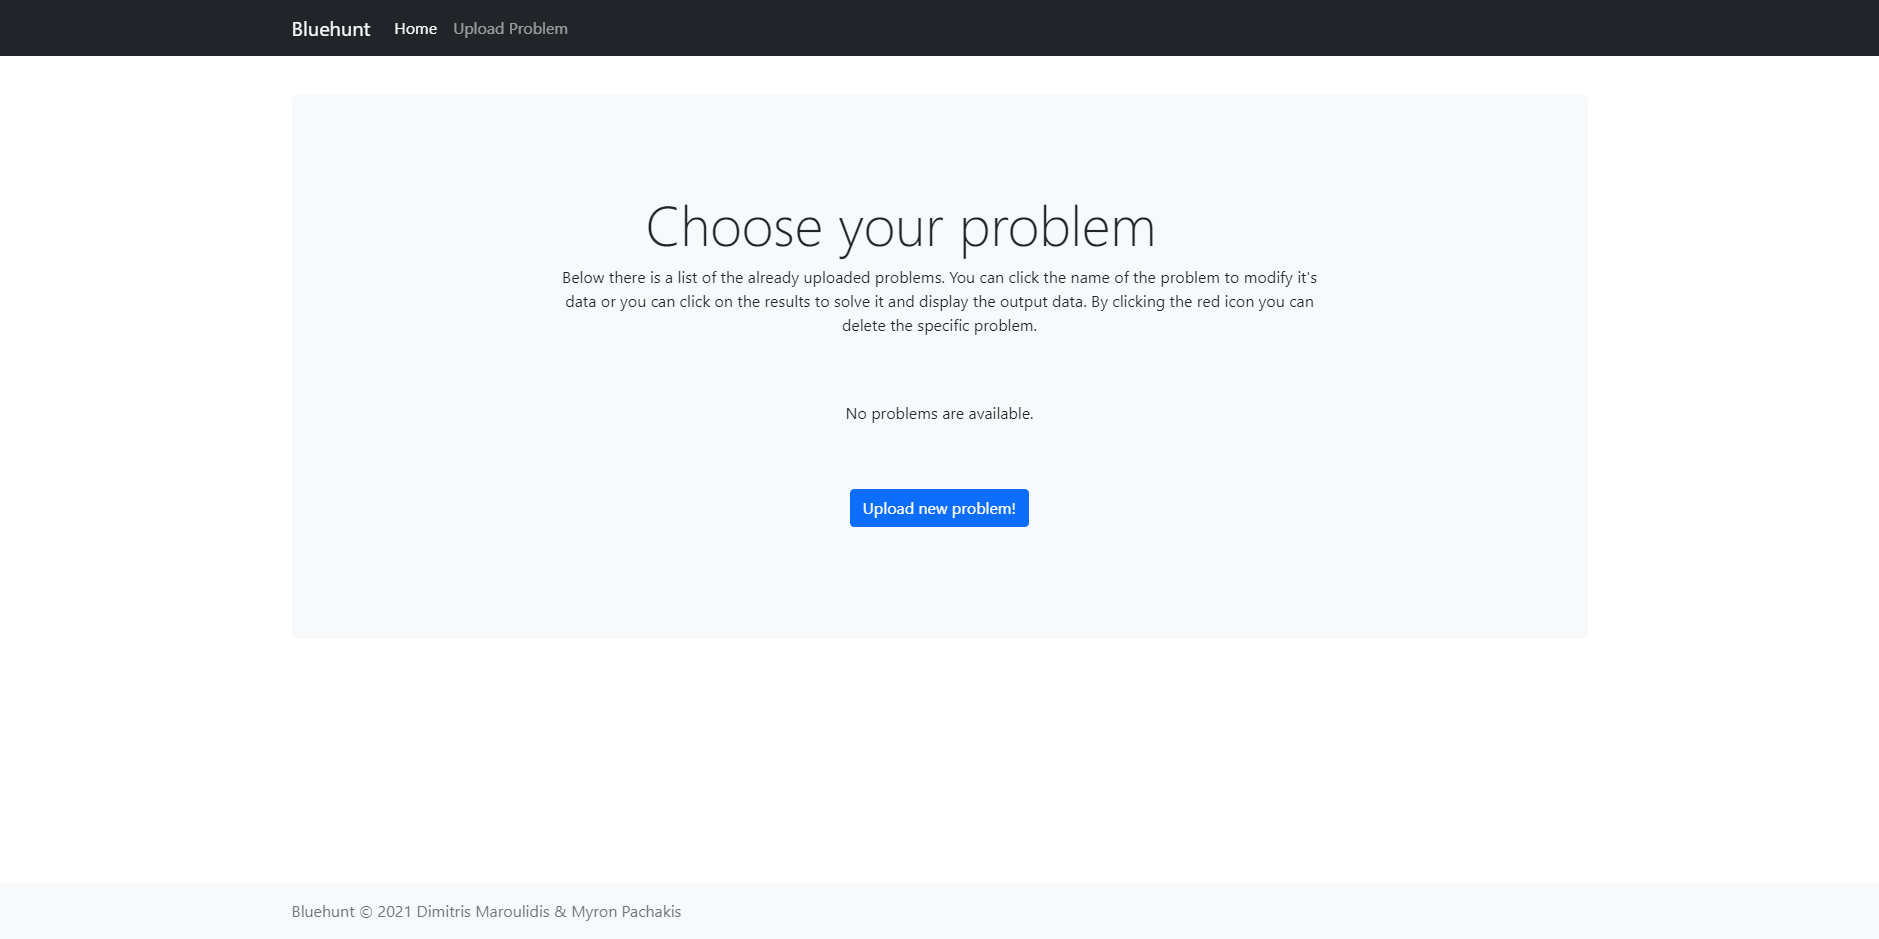
\includegraphics[width=0.8\linewidth]{media/index_no_prob.png}
		\caption{Αρχική σελίδα με κανένα ανεβασμένο πρόβλημα}
		\label{fig:index_no_prob}
	\end{figure}
	
	\begin{figure}[H]
		\centering
		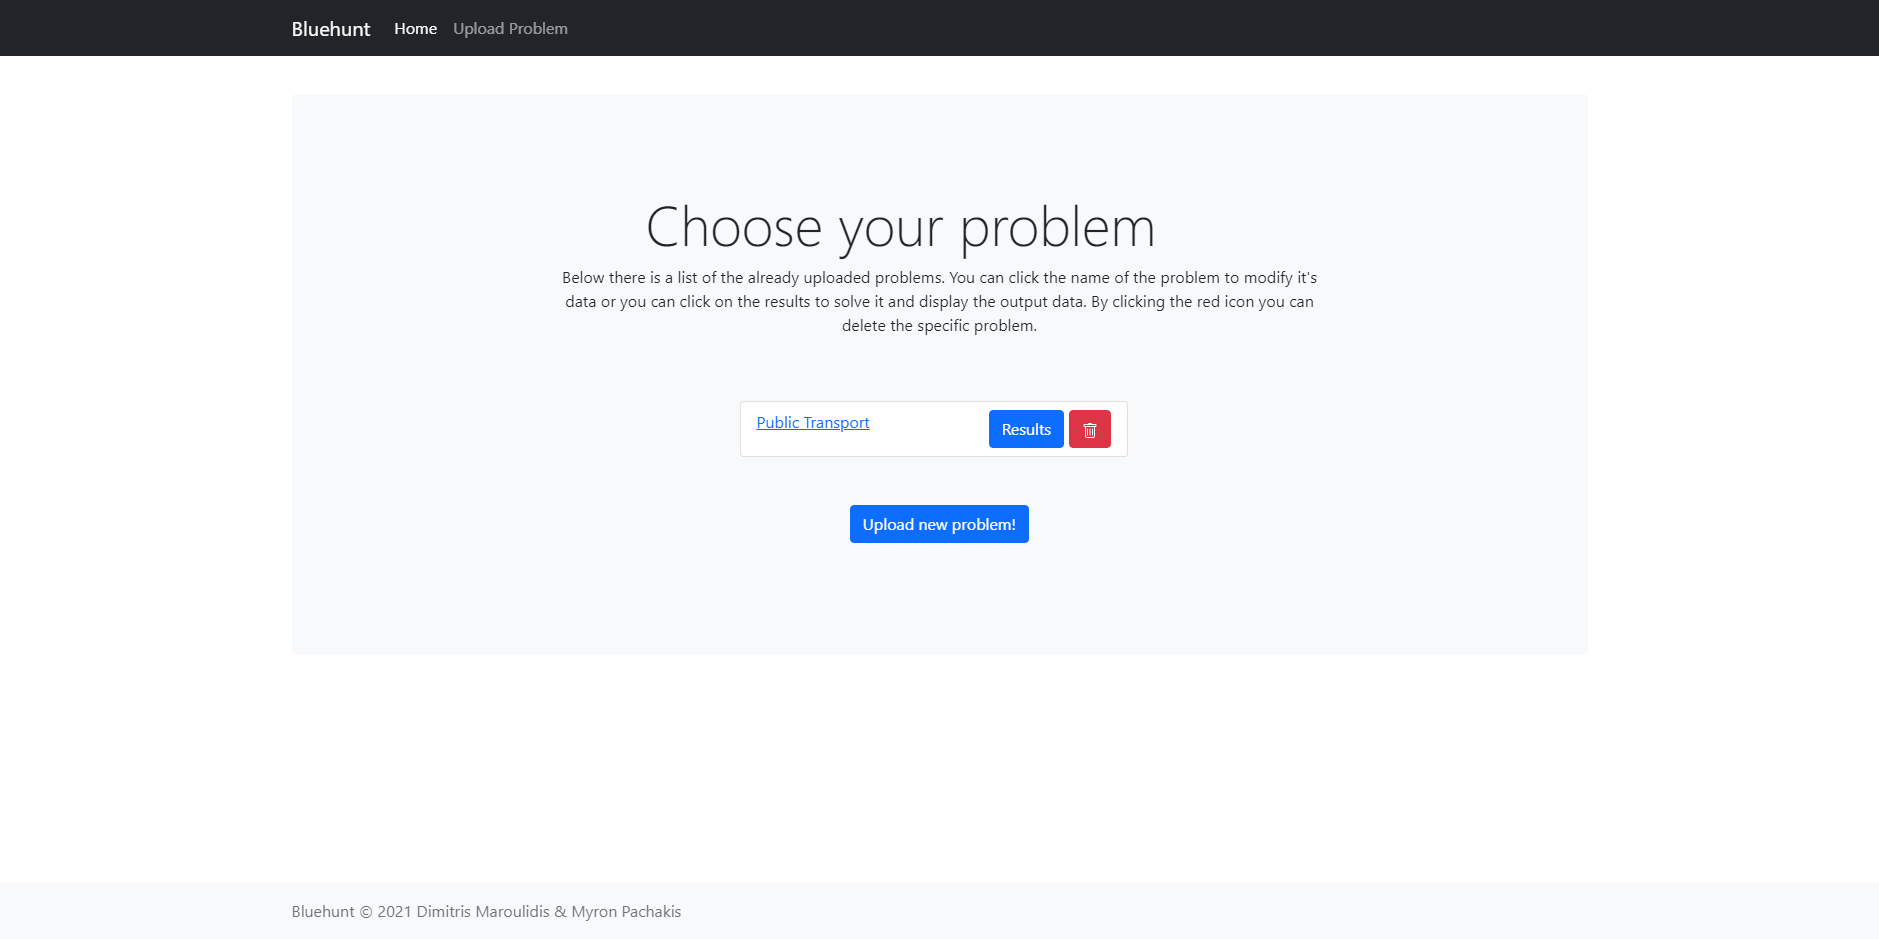
\includegraphics[width=0.8\linewidth]{media/index_with_prob.png}
		\caption{Αρχική σελίδα με ανεβασμένο πρόβλημα}
		\label{fig:index_with_prob}
	\end{figure}
	
	Εάν υπάρχει ήδη ανεβασμένο πρόβλημα τότε πατώντας πάνω στο όνομα του, θα μεταφερθείτε στην σελίδα όπου προβάλονται τα περιεχόμενα του προβλήματος. Με το κουμπί \textbf{Results} παρουσιάζεται αμέσως η λύση του συγκεκριμένου προβλήματος ενώ με το κόκκινο κουμπί διαγράφεται το πρόβλημα από την βάση δεδομένων.
	
	Πατώντας το κουμπί \textbf{Upload new problem!} δημιουργείτε ένα καινούργιο πρόβλημα.
	
	\item Για την δημιουργία του καινούργιου προβλήματος είναι απαραίτητο να ορίσετε ένα όνομα στο πεδίο \textbf{Problem name:} και να επιλέξετε πατώντας το κουμπί \textbf{Choose File} το αρχείο της μορφής Microsoft Excel (.xls, .xlsx) όπου περιέχει τα δεδομένα. Το αρχείο Excel πρέπει να έχει την εξής δομή:
	
	\begin{itemize}
		\item Δύο φύλλα 
		\item Στο πρώτο φύλλο ο πίνακας έχει πρώτη στήλη τα ονόματα των εναλλακτικών, δεύτερη στήλη τη διάταξη των εναλλακτικών και έπειτα, ανάλογα με τα κριτήρια, κάθε στήλη περιέχει τις τιμές των κριτηρίων για κάθε εναλλακτική.
		\item Στο δεύτερο φύλλο ο πίνακας έχει πρώτη στήλη τα ονόματα των κριτηρίων, δεύτερη στήλη την μονοτονικότητα τους (TRUE ή FALSE) και τρίτη στήλη τον αριθμό των υποδιαστημάτων που επιθυμείτε να χωρίσετε σύμφωνα με την εξίσωση \ref{initial_inter}.
	\end{itemize}
	
	\begin{figure}[H]
		\centering
		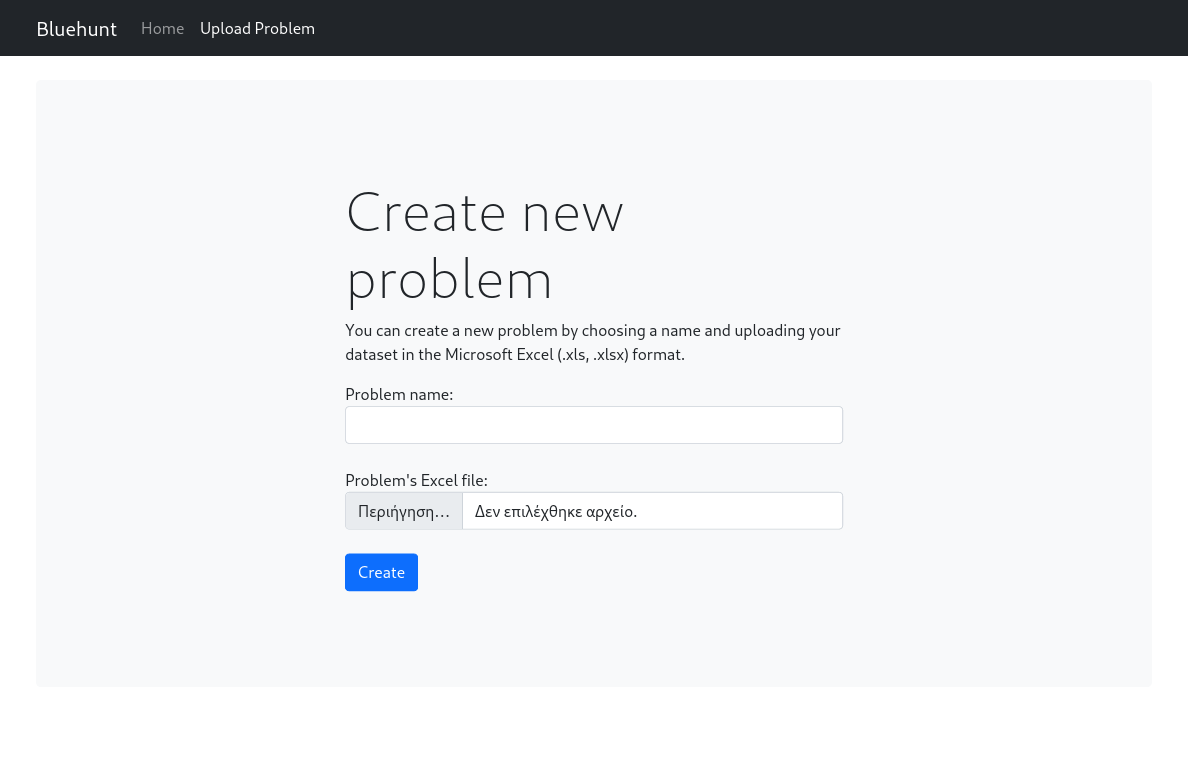
\includegraphics[width=0.8\linewidth]{media/upload.png}
		\caption{Σελίδα για μεταφόρτωση ενός προβλήματος}
		\label{fig:uplaod}
	\end{figure}
	
	\item Πατώντας το κουμπί \textbf{Create} ανακατευθύνεστε στη επόμενη σελίδα όπου παρουσιάζονται τα δεδομένα του προβλήματος που μεταφορτώθηκε καθώς επίσης μπορείτε να αλλάξετε τις μεταβλητές $δ$ και $ε$.
	
	\begin{figure}[H]
		\centering
		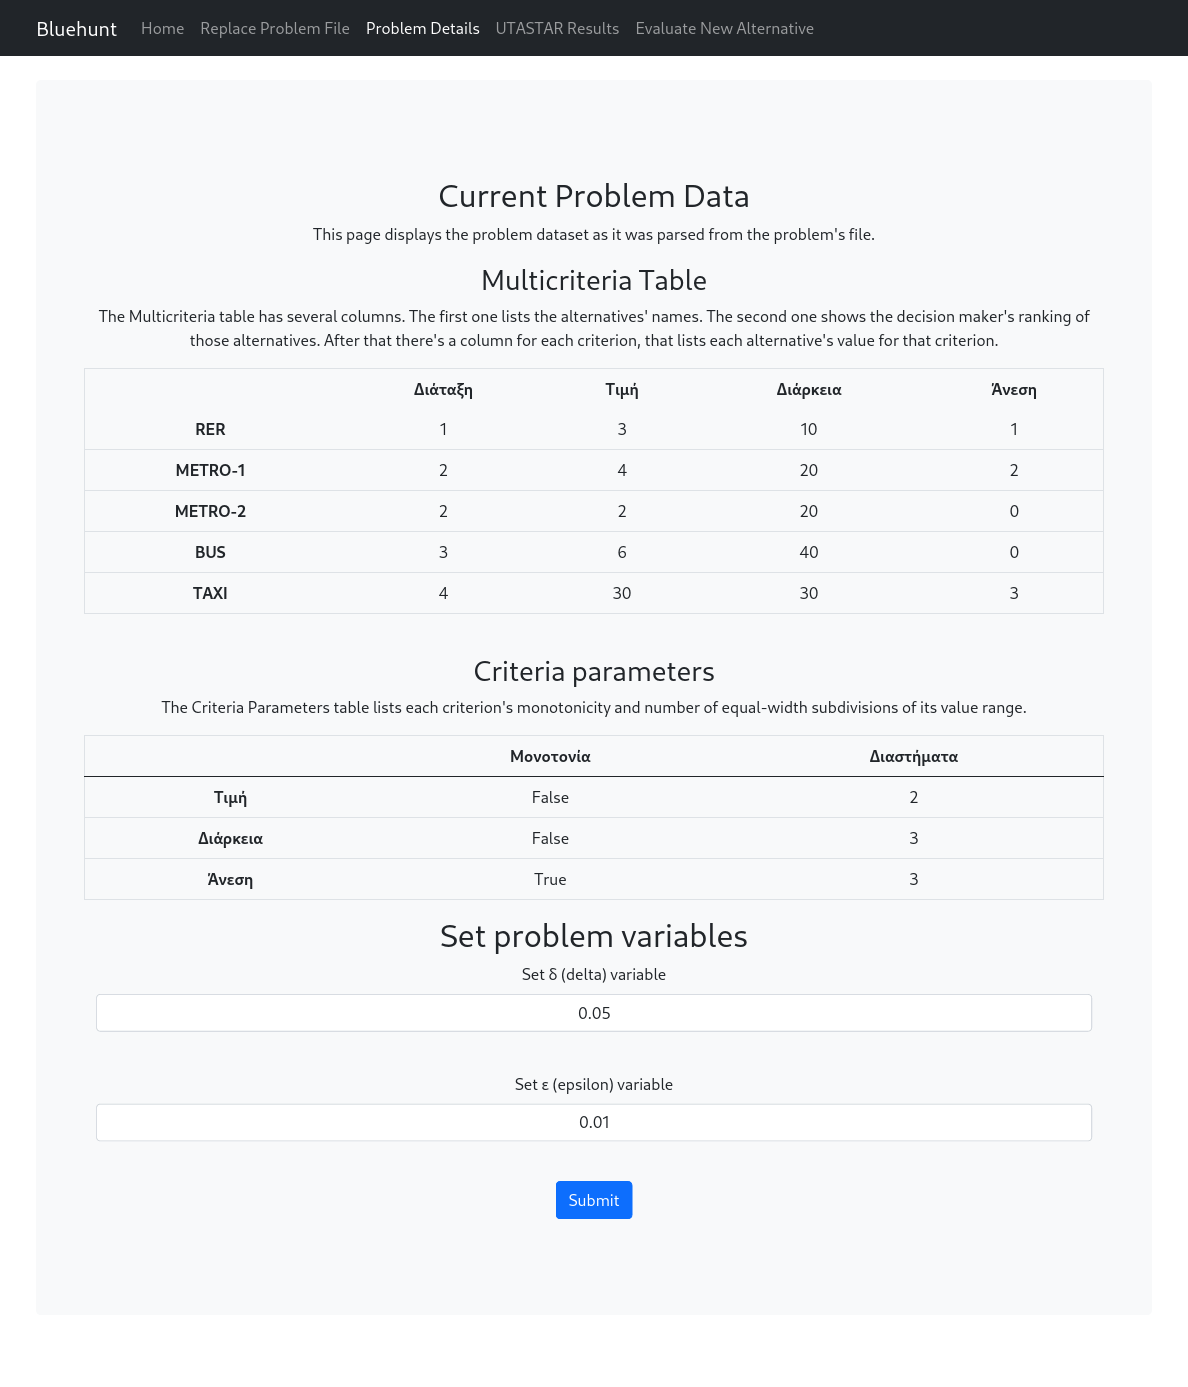
\includegraphics[width=0.8\linewidth]{media/details.png}
		\caption{Σελίδα για προβολή περιεχομένων προβλήματος (συγκεκριμένα τα δεδομένα του προβλήματος των μεταφορικών μέσων)}
		\label{fig:details}
	\end{figure}

	Με το κουμπί \textbf{Submit} θα γίνει επίλυση χρησιμοποιώντας την μέθοδο UTASTAR.
	
	\item Παρουσιάζονται τα αποτελέσματα δηλαδή ο πολυκριτήριος πίνακας με τις τελικές ολικές χρησιμότητες, το $τ$ του Kendall, οι μεταβλητες $w$ του κάθε κριτηρίου και τα διαγράμματα των κανονικοποιημένων μερικών χρησιμοτήτων κάθε κριτηρίου. 
	
	\begin{figure}[H]
		\centering
		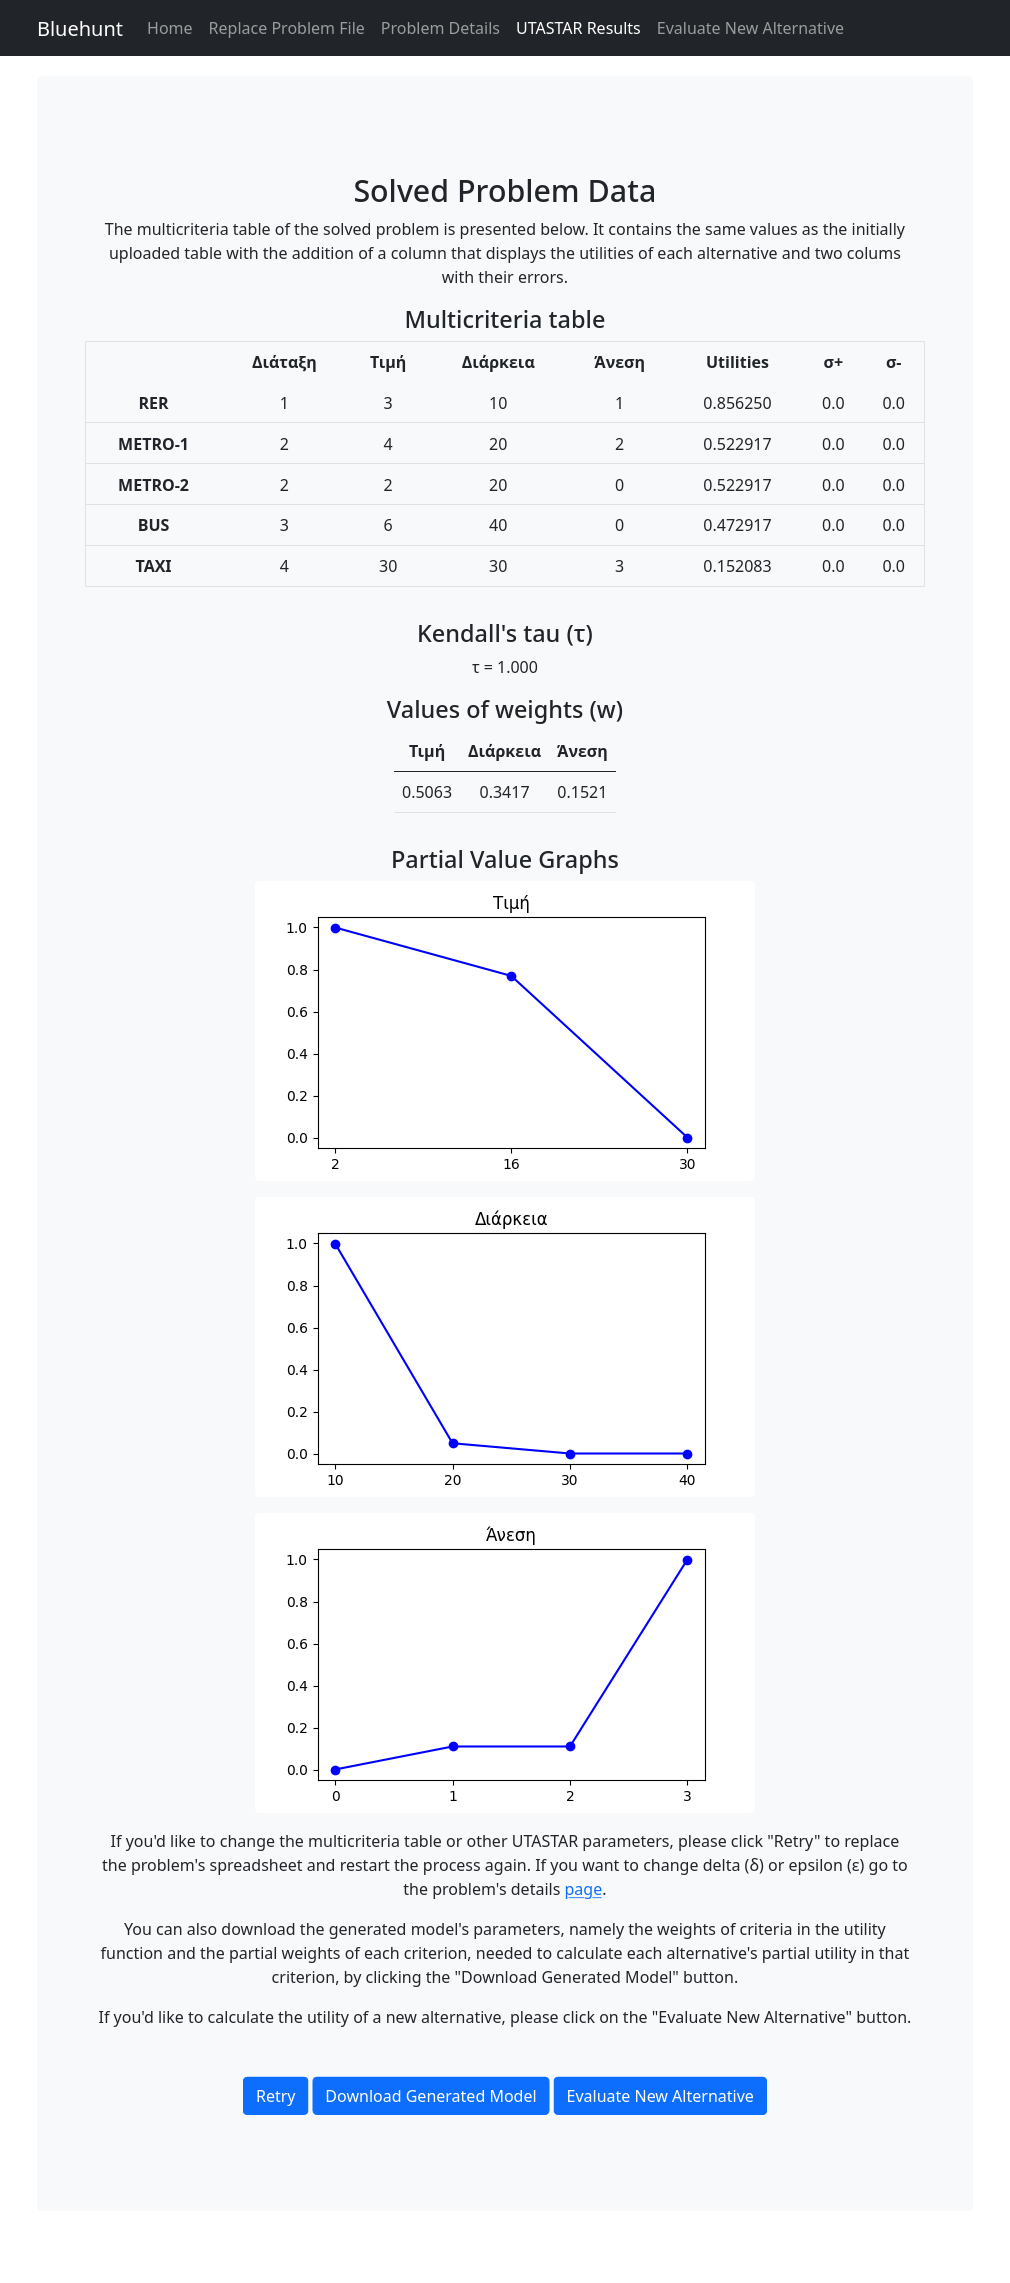
\includegraphics[width=0.8\linewidth]{media/results.png}
		\caption{Τελικός πολυκριτήριος πίνακας, τ του Kendall και διαγράμματα}
		\label{fig:results_1}
	\end{figure}
	

	Στο τέλος υπάρχουν 3 κουμπιά μέσα από τα οποία μπορείτε να κάνετε κάποιες ενέργειες.
	
	\begin{itemize}
		\item Με το κουμπί \textbf{Retry} αντικαθιστάτε το τρέχων αρχείο Excel με κάποιο άλλο.
		
		\begin{figure}[H]
			\centering
			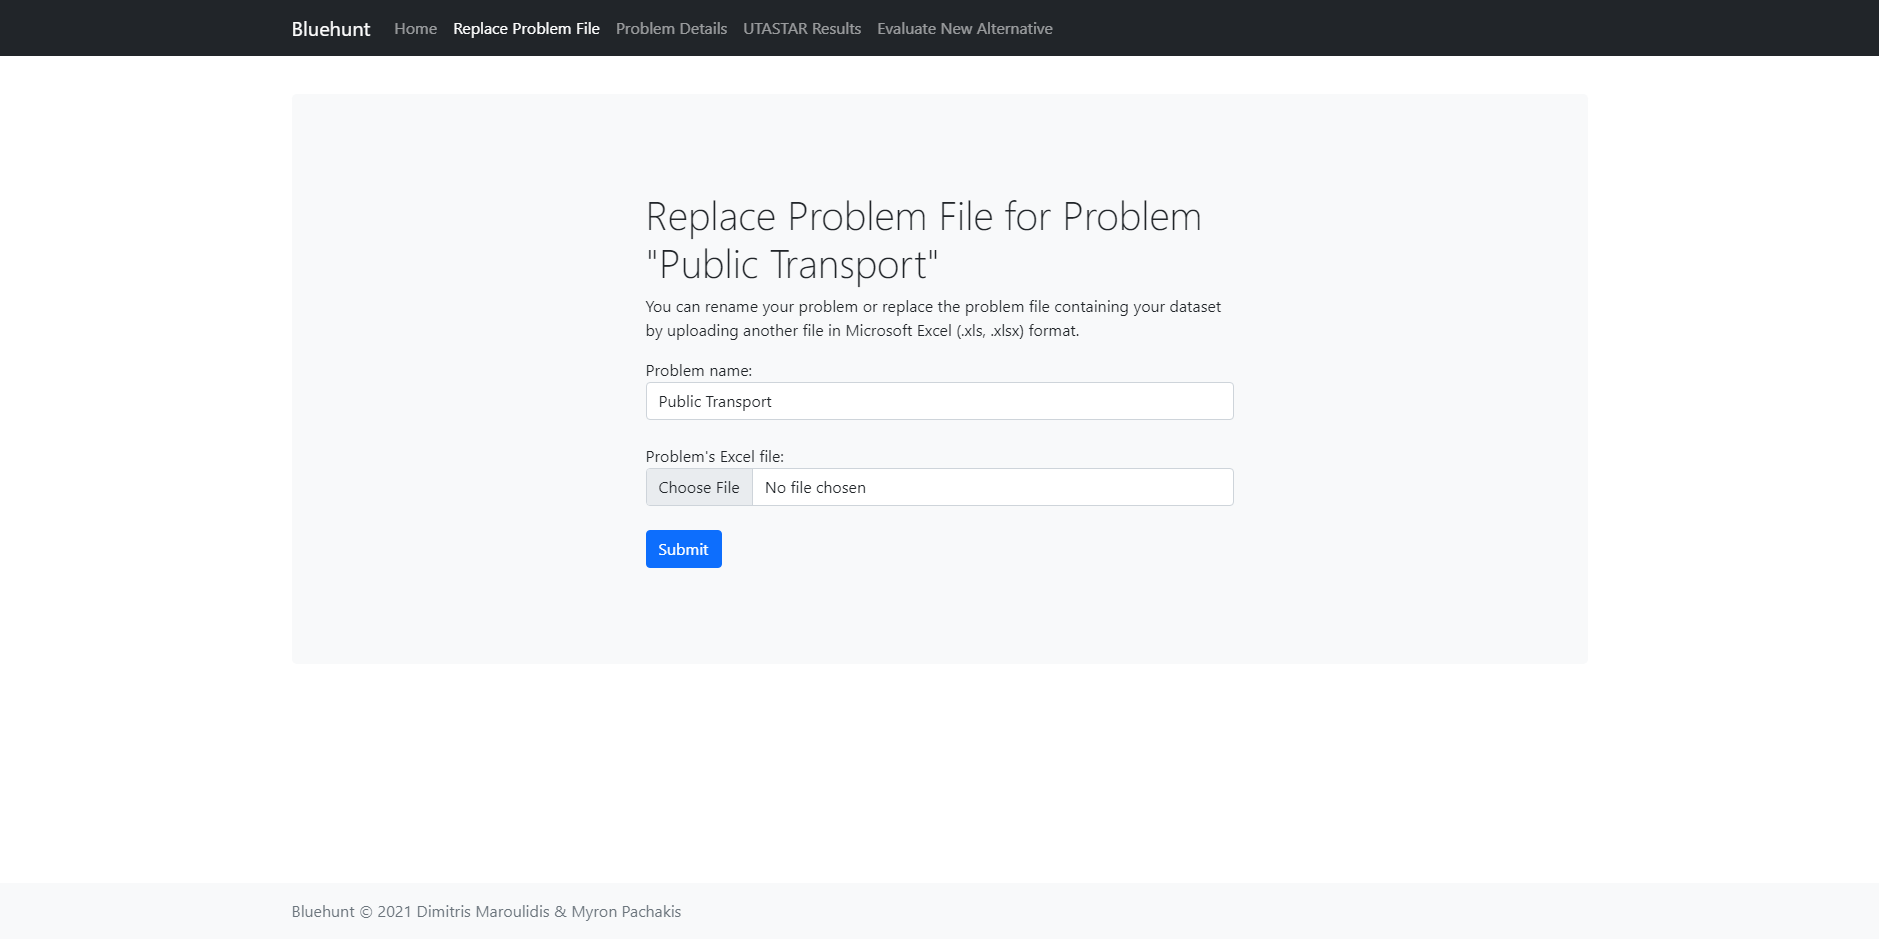
\includegraphics[width=0.8\linewidth]{media/retry.png}
			\caption{Αντικατάσταση αρχείου Excel με άλλο}
			\label{fig:retry}
		\end{figure}
	
		Συμπληρώνετε τα στοιχεία με βάση το βήμα 3.
				
		\item Με το κουμπί \textbf{Download Generated Model} λαμβάνετε τα αποτελέσματα σε μορφή αρχείου Microsoft Excel. 
		\item Με το κουμπί \textbf{Evaluate New Alternative} προσθέτετε επιπλέον εναλλακτική και υπολογίζετε τα ζητούμενα τρέχοντας πάλι την UTASTAR.
		
		\begin{figure}[H]
			\centering
			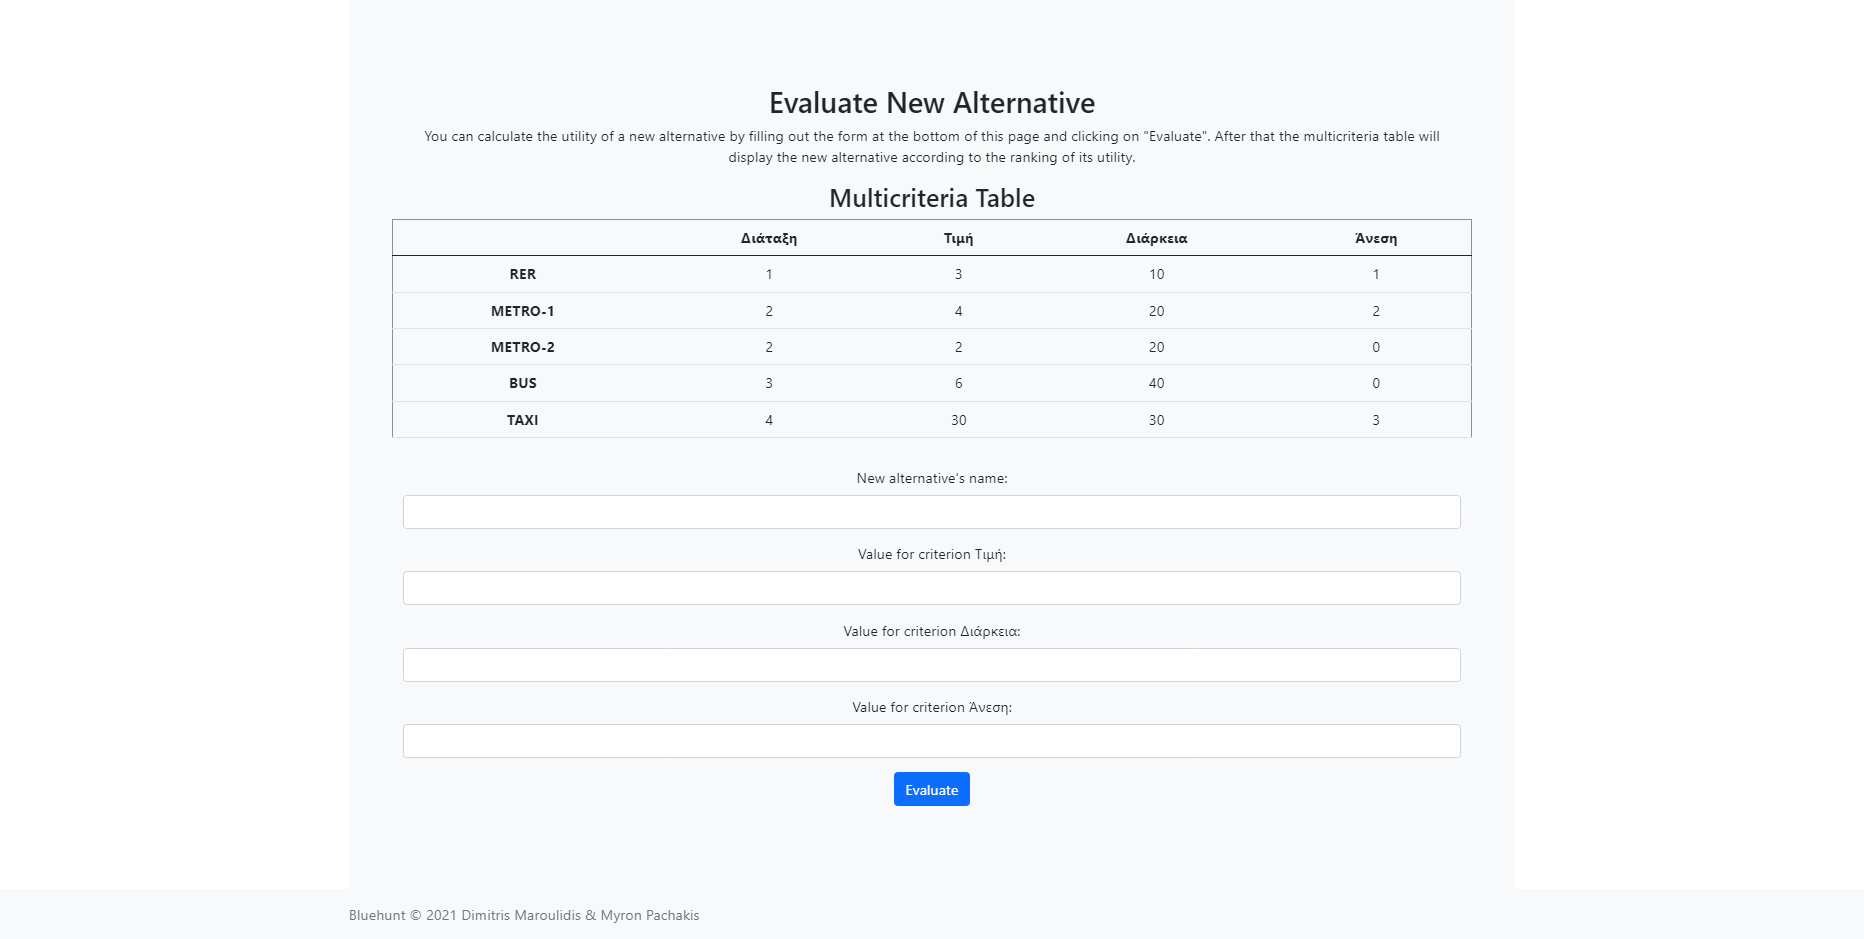
\includegraphics[width=0.8\linewidth]{media/evaluate.png}
			\caption{Προσθήκη επιπλέον εναλλακτικής}
			\label{fig:evaluate}
		\end{figure}
		
		Στο κενό \textbf{New alternative's name:} δίνετε το όνομα της εναλλακτικής και στα κενά \textbf{Value for criterion...:} συμπληρώνετε τη τιμή της συγκεκριμένης εναλλακτικής για κάθε κριτήριο.	
	\end{itemize}
\end{enumerate}

\section{Αναλυτικό Παράδειγμα}
\label{sec:example}

\end{document}